	    \begin{question}{31 et 1215}{Snell-Descartes}{1}{/}
         	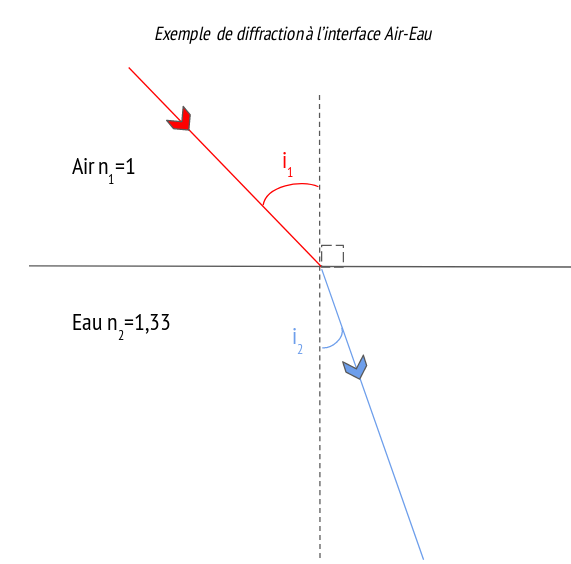
\includegraphics[width=\textwidth]{Christopher/Figures_Christopher/SD_UE.png}
				Quand un rayon lumineux passe d'un milieu à un autre (par exemple de l'air à l'eau), sa trajectoire change : son angle d'arrivée n'est pas le même que celui de sortie. La loi de Snell-Descartes permet de décrire ce phénomène en reliant les indices optiques $n_1$ et $n_2$ des deux milieux ainsi que les angles  $i_1$ et  $i_1$ des rayons incident et réfracté, avec la relation suivante  : $n_1\sin(i_1)=n_2\sin(i_2)$. Parmi les propositions suivantes, trouver celle qui décrit la loi de Snell-Descartes : 
            \end{question}
            \begin{reponses}
            	\item[false] $\frac{sin(i_1)}{n_1}=\frac{sin(i_2)}{n_2}$
            	\item[false] $\frac{n_2}{n_1}=\frac{sin(i_2)}{sin(i_1)}$
                \item[true] $\frac{sin(i_2)}{sin(i_1)}=\frac{n_1}{n_2}$
                \item[false] $\frac{n_1}{sin(i_1)}=\frac{n_2)}{sin(i_2)}$
            \end{reponses}
			%%%%%%%%%%%%%%%%%%%%%%%%%%%%%%%%%%%%%
        	\begin{question}{31 et 1215}{Snell-Descartes}{2}{/}
				Envoyons un rayon lumineux (on se placera dans l'air d'indice $n_1$=1) sur une solution transparente d'indice $n_2$ inconnu. L'angle d'incidence $i_1$ est de $30\si\degree$ et l'angle réfracté mesuré $i_2$ est de $20\si\degree$. En utilisant la loi de Snell-Descartes, déterminer l'indice $n_2$.
            \end{question}
            \begin{reponses}
            	\item[false] 1,08
            	\item[true]  1,46
                \item[false] 0,68
                \item[false] 81
                \item[false] 0,17
            \end{reponses}
			%%%%%%%%%%%%%%%%%%%%%%%%%%%%%%%%%%%%%  
            \begin{question}{31 et 1215}{Snell-Descartes}{2}{/}
				Envoyons un rayon lumineux (on se placera dans l'air d'indice $n_1$=1) sur une solution transparente d'indice $n_2$ inconnu. L'angle d'incidence $i_1$ est de $\frac{\pi}{3} \si\radian$ et l'angle réfracté mesuré $i_2$ est de $\frac{\pi}{6} \si\radian$. En utilisant la loi de Snell-Descartes, déterminer l'indice $n_2$.
            \end{question}
            \begin{reponses}
            	\item[true] $\sqrt[]{3}$ 
            	\item[false] $\frac{3}{2}$
                \item[false] $\frac{1}{2}$
                \item[false] 2
                 \item[false] $\frac{\sqrt[]{3}}{2}$
            \end{reponses}
			%%%%%%%%%%%%%%%%%%%%%%%%%%%%%%%%%%%%%  
            \begin{question}{31 et 1215}{Snell-Descartes}{2}{/}
				Envoyons un rayon lumineux (on se placera dans l'air d'indice $n_1$=1) sur une solution transparente d'indice $n_2=1.41$. L'angle d'incidence $i_1$ est de $\SI{45}{\degree}$ et l'angle réfracté mesuré $i_2$ est inconnu. En utilisant la loi de Snell-Descartes, déterminer l'angle $i_2$.
            \end{question}
            \begin{reponses}
            	\item[false]$\SI{45}{\degree}$
            	\item[false] $\SI{60}{\degree}$
                \item[true] $\SI{30}{\degree}$
                \item[false] $\SI{90}{\degree}$
            \end{reponses}
			%%%%%%%%%%%%%%%%%%%%%%%%%%%%%%%%%%%%%
